\noindent
\begin{minipage}[t]{0.48\textwidth}
  \secrule\vspace{0.35em}
  {\color{stewartcyan}\textbf{25--26}}\enspace Coi $y$ là biến độc lập và $x$ là biến phụ thuộc, hãy sử dụng đạo hàm ẩn để tìm $dx/dy$.
  \vspace{0.4em}

  \noindent
  \textbf{25.}\enspace $x^4y^2 - x^3y + 2xy^3 = 0$ \hfill \textbf{26.}\enspace $y\sec x = x\tan y$
  \vspace{0.3em}

  \noindent\secrule\vspace{0.35em}

  \noindent
  {\color{stewartcyan}\textbf{27--36}}\enspace Sử dụng đạo hàm ẩn để tìm phương trình tiếp tuyến của đường cong tại điểm đã cho.
  \vspace{0.4em}

  \noindent
  \textbf{27.}\enspace $ye^{\sin x} = x\cos y, \quad (0, 0)$
  \vspace{0.3em}

  \noindent
  \textbf{28.}\enspace $\tan(x + y) + \sec(x - y) = 2, \quad (\pi/8, \pi/8)$
  \vspace{0.3em}

  \noindent
  \textbf{29.}\enspace $x^{2/3} + y^{2/3} = 4, \quad (-3\sqrt{3}, 1) \quad\text{(đường astroid)}$
  \vspace{0.3em}

  \noindent
  \textbf{30.}\enspace $y^2(6 - x) = x^3, \quad (2, \sqrt{2}) \quad\text{(đường cissoid của Diocles)}$
  \vspace{0.3em}

  \noindent
  \textbf{31.}\enspace $x^2 - xy - y^2 = 1, \quad (2, 1) \quad\text{(hyperbol)}$
  \vspace{0.3em}

  \noindent
  \textbf{32.}\enspace $x^2 + 2xy + 4y^2 = 12, \quad (2, 1) \quad\text{(elip)}$
  \vspace{0.3em}

  \noindent
  \textbf{33.}\enspace $x^2 + y^2 = (2x^2 + 2y^2 - x)^2, \quad (0, \frac{1}{2}) \quad\text{(đường cardioid)}$
  \begin{center}
    \vspace{-0.2em}
    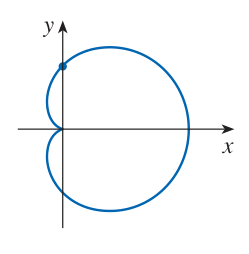
\includegraphics[width=0.40\linewidth]{images/p0250_fig1.png}
    \vspace{-0.3em}
  \end{center}

  \noindent
  \textbf{34.}\enspace $x^2y^2 = (y + 1)^2(4 - y^2), \quad (-2\sqrt{3}, 1)$\\
  \phantom{\textbf{34.}\enspace}\text{(đường conchoid của Nicomedes)}
  \begin{center}
    \vspace{-0.2em}
    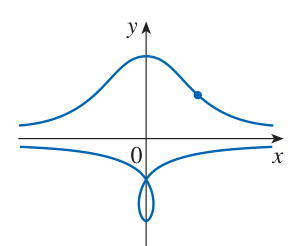
\includegraphics[width=0.50\linewidth]{images/p0250_fig2.png}
    \vspace{-0.3em}
  \end{center}

  \noindent
  \textbf{35.}\enspace $2(x^2 + y^2)^2 = 25(x^2 - y^2), \quad (3, 1) \quad\text{(đường lemniscate)}$
  \begin{center}
    \vspace{-0.2em}
    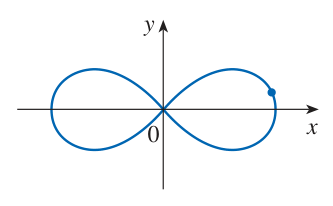
\includegraphics[width=0.50\linewidth]{images/p0250_fig3.png}
    \vspace{-0.3em}
  \end{center}

  \noindent
  \textbf{36.}\enspace $y^2(y^2 - 4) = x^2(x^2 - 5), \quad (0, -2) \quad\text{(đường cong quỷ)}$
  \begin{center}
    \vspace{-0.2em}
    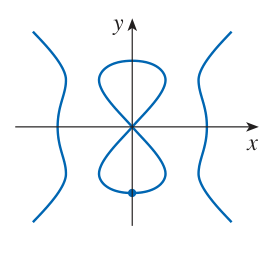
\includegraphics[width=0.42\linewidth]{images/p0250_fig4.png}
    \vspace{-0.3em}
  \end{center}

  \noindent\secrule
\end{minipage}%
\hfill
\begin{minipage}[t]{0.48\textwidth}
  \noindent
  \textbf{37.}\enspace (a) Đường cong có phương trình $y^2 = 5x^4 - x^2$ được gọi là \textbf{kampyle của Eudoxus}. Tìm một phương trình tiếp tuyến của đường cong này tại điểm $(1, 2)$.\\[0.3em]
  \makebox[0pt][r]{\graphicon\enspace}(b) Minh họa phần (a) bằng cách vẽ đồ thị của đường cong và tiếp tuyến trên cùng một màn hình. (Vẽ đường cong được xác định ẩn nếu có thể, hoặc bạn có thể vẽ riêng biệt hai nửa trên và dưới.)
  \vspace{0.45em}

  \noindent
  \textbf{38.}\enspace (a) Đường cong có phương trình $y^2 = x^3 + 3x^2$ được gọi là \textbf{đường bậc ba Tschirnhausen}. Tìm một phương trình tiếp tuyến của đường cong này tại điểm $(1, -2)$.\\[0.3em]
  (b) Tại những điểm nào thì đường cong này có tiếp tuyến nằm ngang?\\[0.3em]
  \makebox[0pt][r]{\graphicon\enspace}(c) Minh họa các phần (a) và (b) bằng cách vẽ đồ thị của đường cong và các tiếp tuyến trên cùng một màn hình.
  \vspace{0.45em}

  \noindent\secrule\vspace{0.35em}
  {\color{stewartcyan}\textbf{39--42}}\enspace Tìm $y''$ bằng đạo hàm ẩn. Rút gọn nếu có thể.
  \vspace{0.35em}

  \noindent
  \textbf{39.}\enspace $x^2 + 4y^2 = 4$ \hfill \textbf{40.}\enspace $x^2 + xy + y^2 = 3$\\[0.35em]
  \textbf{41.}\enspace $\sin y + \cos x = 1$ \hfill \textbf{42.}\enspace $x^3 - y^3 = 7$
  \vspace{0.25em}

  \noindent\secrule\vspace{0.45em}

  \noindent
  \textbf{43.}\enspace Nếu $xy + e^y = e$, hãy tìm giá trị của $y''$ tại điểm có $x = 0$.
  \vspace{0.45em}

  \noindent
  \textbf{44.}\enspace Nếu $x^2 + xy + y^3 = 1$, hãy tìm giá trị của $y'''$ tại điểm có $x = 1$.
  \vspace{0.45em}

  \noindent
  \makebox[0pt][r]{\graphicon\enspace}\textbf{45.}\enspace Các hình dạng kỳ thú có thể được tạo ra bằng cách sử dụng phần mềm có khả năng vẽ đồ thị các đường cong được xác định ẩn.\\[0.3em]
  (a) Vẽ đồ thị đường cong có phương trình
  \[ y(y^2 - 1)(y - 2) = x(x - 1)(x - 2) \]
  Tại bao nhiêu điểm thì đường cong này có tiếp tuyến nằm ngang? Hãy ước lượng hoành độ $x$ của các điểm này.\\[0.3em]
  (b) Tìm phương trình các tiếp tuyến tại các điểm $(0, 1)$ và $(0, 2)$.\\[0.3em]
  (c) Tìm hoành độ $x$ chính xác của các điểm trong phần (a).\\[0.3em]
  (d) Tạo ra các đường cong kỳ thú hơn nữa bằng cách biến đổi phương trình ở phần (a).
  \vspace{0.45em}

  \noindent
  \makebox[0pt][r]{\graphicon\enspace}\textbf{46.}\enspace (a) Đường cong có phương trình
  \[ 2y^3 + y^2 - y^5 = x^4 - 2x^3 + x^2 \]
  được ví như một chiếc xe ngựa nhún nhảy. Hãy vẽ đồ thị đường cong này và khám phá lý do tại sao.\\[0.3em]
  (b) Tại bao nhiêu điểm thì đường cong này có các tiếp tuyến nằm ngang? Tìm hoành độ $x$ của các điểm này.
  \vspace{0.45em}

  \noindent
  \textbf{47.}\enspace Tìm các điểm trên đường lemniscate trong Bài tập 35 mà tại đó tiếp tuyến nằm ngang.
  \vspace{0.45em}

  \noindent
  \textbf{48.}\enspace Sử dụng đạo hàm ẩn để chứng minh rằng tiếp tuyến của elip
  \[ \frac{x^2}{a^2} + \frac{y^2}{b^2} = 1 \]
  tại điểm $(x_0, y_0)$ có phương trình là
  \[ \frac{x_0x}{a^2} + \frac{y_0y}{b^2} = 1 \]
\end{minipage}

\vfill
\begin{center}
  \fontsize{6.5pt}{8pt}\selectfont\color{gray!80}
  Copyright 2021 Cengage Learning. All Rights Reserved. May not be copied, scanned, or duplicated, in whole or in part. WCN 02-200-203\\
  Bản quyền thuộc về Cengage Learning. Bản dịch tiếng Việt phục vụ mục đích học tập và nghiên cứu.
\end{center}
